% !Mode:: "TeX:UTF-8" 

\BiChapter{决策模型}{4}
\BiSection{离线强化学习}{}\label{sec-offline-rl}
离线强化学习(Offline Reinforcement Learning)是指在没有与环境交互的情况下,
使用预先手机的随机或专家数据来训练强化学习算法,这类算法适用于无法频繁与环境交互或交互代价高昂的场景,
例如自动驾驶、机器人控制等。由于本任务中的非嵌入环境,与环境交互速度效率很低,所以考虑使用离线强化学习作为决策模型。

首先对强化学习中的概念进行介绍,
考虑无限长度的Markov决策过程(MDP),定义为$(\mathcal{S},\mathcal{A},p,r,\rho_0)$,
其中$\mathcal{S}$为状态空间,$\mathcal{A}$为动作空间,
$p:\mathcal{S}\times \mathcal{A}\times \mathcal{S}\to \mathbb{R}$为状态转移方程,
$r:\mathcal{S}\to \mathbb{R}$为奖励函数,$\rho_0:\mathcal{S}\to \mathbb{R}$为初始状态$s_0$对应的分布。

令$\pi$表示决策函数$\pi: \mathcal{S}\times \mathcal{A}\to [0,1]$,令$R(\pi)$表示其期望所获得的总奖励(回报):
\begin{equation}
  R(\pi) = \mathbb{E}_{S_1,A_1,S_2,A_2\cdots}\left[\sum_{t=0}^{\infty}r(S_t)\right],\quad
  \text{~其中~}S_1\sim\rho_0(\cdot),A_t\sim\pi(\cdot|S_t),S_{t+1}\sim p(\cdot|S_t,A_t)
\end{equation}
强化学习的目标通常是找到最优策略$\pi^* := \argmax_{\pi}R(\pi)$,
在线强化学习算法往往通过策略迭代和价值函数估计方法实现策略的更新,
而下文中所使用的离线强化学习算法不再基于值估计方法,而是更加类似于模仿学习的方法。

\BiSubsection{Decision Transformer}{}
Decision Transformer(DT)\upcite{DT}是一种将强化学习问题是为序列建模问题的方法,使用了深度学习中的Transformer架构,
对于离线数据集中的一段长度为$T$的交互轨迹(Trajectory)
\begin{equation}
  \tau = (s_1,a_1,r_1,s_2,a_2,r_2,\cdots,s_T,a_T,r_T,s_{T+1})
\end{equation}
其中$s_{T+1}$为终止状态,则$\rho$可以视为建模为序列
\begin{equation}\label{eq-sequence}
  R_0,s_1,a_1,R_1,s_2,\cdots,a_{T-1},R_{T-1},s_{T},a_{T}
\end{equation}
其中$R_i=\sum_{t=i}^Tr_{t+1}, \quad(i=0,\cdots,T-1)$为目标回报(Return-to-Go)。

DT模型中序列编码模型使用的是GPT模型\upcite{GPT},即仅含有编码器的因果注意力机制。
具体来讲,假设当前处理的序列$X\in\mathbb{R}^{d\times N}$长度为$N$,每个特征编码维度为$d$,
则注意力机制\upcite{attention}包含三个可学习矩阵$Q_{\theta},K_{\theta}\in\mathbb{R}^{d_k\times d}, V_{\theta}\in\mathbb{R}^{d_v\times d}$,
分别对应生成询问键(Query),查询键(Key)和价值键(Value)
\begin{equation}
  Q=Q_{\theta}X,\quad K=K_{\theta}X,\quad V=V_{\theta}X,
\end{equation}
则对于序列中第$i\in\{1,\cdots,N\}$个特征对应的\textbf{交叉注意力(Cross-Attention)}为
\begin{equation}
  \bd{z}^{cross}_i = \sum_{j=1}^N\text{softmax}\left(\left\{\frac{1}{\sqrt{d_k}}\langle \bd{q}_i,\bd{k}_l\rangle\right\}_{l=1}^N\right)_j\cdot \bd{v}_j\iff
  Z^{cross} = \text{softmax}\left(\frac{QK^T}{\sqrt{d_k}}\right)V
\end{equation}
其中包含系数$1/\sqrt{d_k}$的原因:不妨假设$\bd{q}_{ij},\bd{k}_{lj}\sim \mathcal{N}(0,\sigma^2),~(j\in\{1,\cdots,d_k\})$,
则$\sum_{j=1}^{d_k}\bd{q}_{ij}\bd{k}_{lj}\sim\mathcal{N}(0,d_k\sigma^2)$,由于初始化的神经网络输出可以保证$\sigma\approx 1$,
因此使用系数$1/\sqrt{d_k}$可以保持输出的方差在$1$左右,避免发散。

\textbf{因果注意力(Causal-Attention)}为(每个特征$i$只能看到$j\leqslant i$的特征)
\begin{align}
  &\ \bd{z}^{causal}_i = \sum_{j=1}^i\text{softmax}\left(\left\{\frac{1}{\sqrt{d_k}}\langle \bd{q}_i,\bd{k}_l\rangle \right\}_{l=1}^N\right)_j\cdot \bd{v}_j\\
  \iff &\ Z^{causal} = \text{softmax}\left(\frac{\left(QK^T\right)\odot M}{\sqrt{d_k}}\right)V,\quad
  \text{~其中~}M\text{~为~}N\text{~阶下三角阵~}\label{eq-causal-attn}
\end{align}
引入因果注意力机制后,每个特征由于无法观察到后续特征,所以可以对相邻的下一个特征进行预测,
从而无需再对编码器和解码器进行区分,降低了代码复杂性。

DT训练方法:首先从离线数据集中随机采样得到一段长度为$N$的轨迹
\begin{equation}
  \tau_{t-N+1:t} =: (s_1,a_1,r_1,s_2,a_2,r_2,\cdots,s_N,a_N,r_N) = \{(s_n,a_n,R_n)\}_{n=1}^N
\end{equation}

再每个特征编码到相同维度$\mathbb{R}^d$下,按式~\ref{eq-sequence}
建模为长度$3N$的序列$\tau\in\mathbb{R}^{3N\times d}$,用GPT模型对序列进行特征编码可以得到和$\tau$维度相同的编码序列$\tau'$,
再取出状态序列所对应的编码结果,通过线性变换映射到动作空间维度,从而得到对相邻动作的预测
\begin{equation}
  \tau'_2,\tau'_5,\cdots, \tau'_{3k-1},\cdots,\tau'_{3N-1}\xrightarrow{\text{~线性变换~}}
  \hat{a}_1,\hat{a}_2,\cdots, \hat{a}_{k},\cdots, \hat{a}_{N}
\end{equation}

对于离散动作空间使用定义~\ref{def-cross-entropy}~中的多元交叉熵损失,
连续动作空间则使用$\ell^2$范数(Mean Square Error, MSE)作为损失函数。

DT验证方法:需给出模型期望达到的总奖励$\hat{R}_0$,通过自迭代的方式时模型完成动作预测,
具体来说,假设初始状态为$s_1$,则初始轨迹为$\tau_1=(\hat{R}_0,s_1)$,模型对$\tau_1$进行编码,
取出最后一个状态$s_1$所对应的预测动作$\hat{a}_1$与环境交互,
得到新的状态$s_2$和奖励$r_1$,令$\hat{R}_1 = \hat{R}_0 - r_1$,
从而得到新的序列$\tau_2 = (\hat{R}_0,s_1,\hat{a}_1, \hat{R}_1, s_2)$,模型再对$\tau_2$进行编码,
取出$s_2$所对应的预测动作$\hat{a}_2$与环境交互,以此类推,直到环境达到终止状态为止。
这种方式和自然语言模型中文本生成的做法基本一致。

\BiSubsection{StARformer}{}\label{sec-starformer}
StARformer\upcite{StARformer}是一种基于ViT\upcite{ViT}专门对状态中的图像特征编码进行的改进,
通过将轨迹$\tau$中的$\{(a_{n-1},r_{n-1},s_{n})\}_{n=1}^{3N}$($a_0$使用特征填充补全)
按照空间维度进行展开($s_{n}$使用图像分块的方法将图像分块序列化),
并压缩到空间特征维度$d'$,进而在\textbf{空间维度}上使用交叉注意力机制进行编码,
得到$\{(a'_{n-1},r'_{n-1},s'_{n})\}_{n=1}^{3N}$,
再将第$n$时刻对应的编码$(a'_{n-1},r'_{n-1},s'_{n})$全部展平,
使用线性变换到时间维度$\mathbb{R}^d$中,将其记为$\{l_{n}\}_{n=1}^N$,
则\textbf{时间维度}的序列建模为
\begin{equation}
  \tau:=s_1,l_1,s_2,l_2,\cdots,s_N,l_N
\end{equation}

通过因果注意力机制(相邻的$(s_n,l_n),~n=1,\cdots,N$之间仍然具有注意力机制)可以完成对时序序列信息的编码,
将编码结果记为$\tau'$,
类似DT的预测方法,只考虑所有状态对应的编码结果,
通过线性变换映射到动作空间维度,从而得到相邻动作的预测
\begin{equation}
  \tau'_1,\tau'_3,\cdots, \tau'_{2k-1},\cdots,\tau'_{2N-1}\xrightarrow{\text{~线性变换~}}
  \hat{a}_1,\hat{a}_2,\cdots, \hat{a}_{k},\cdots, \hat{a}_{N}
\end{equation}
模型的训练及推理方式与DT完全一致,相比DT模型,StARformer能够有效的提高模型对图像信息的理解能力,
本毕设对上述离线强化学习算法进行了复现\footnote{\url{https://github.com/wty-yy/Decision-Transformer-JAX},
复现内容包括:Decision Transformer(DT),Return-Aligned Decision Transformer(RADT)和StARformer,
在Atari环境中进行了对比试验,并对结果进行可视化。},本文的相关复现实验显示
相比DT更不依赖于初始时目标总奖励$\hat{R}_0$的设定,这说明其更倾向于对专家数据的模仿学习,而非与目标总奖励进行对齐,
在5个不同Atari环境下的实验表明,StARformer的平均得分超过DT算法的$30\%$。

\BiSection{决策模型设计}{}\label{sec-model}
\BiSubsection{状态空间与动作空间}{}
模型的状态输入由2部分构成,分别为$S^{img}, \bd{s}^{card}$,其中$S^{img}\in\mathbb{R}^{18\times 32\times 15}$为单位的网格状特征输入,
对于第$i$行$j$列的特征$\bd{z}_{ij}:=(S^{img})_{ij}\in\mathbb{R}^{15}$
表示处于该位置的单位具有如下$4$种特征:$(\bd{z}_{ij})_{1:8}$为类别编码,
$(\bd{z}_{ij})_9$为从属派别编码,$(\bd{z}_{ij})_{10:12}$为生命值图像编码,$(\bd{z}_{ij})_{13:15}$为其余条状图像编码;
$\bd{s}^{card}\in\mathbb{R}^6$表示当前状态下的两个全局特征:$(\bd{s}^{card})_{1:5}$为当前手牌信息,
$(\bd{s}^{card})_6$为当前总圣水量。

模型的动作输入由2个部分构成:$\bd{a}^{pos}, a^{select}$,其中$\bd{a}^{pos}\in\mathbb{R}^2$表示动作执行的部署坐标,
$a^{select}$表示动作执行的手牌编号。

\BiSubsection{预测目标设计与重采样}{}\label{sec-target}
由于本任务中动作执行极为离散,总帧数中仅有$4\%$为执行动作帧,其余帧均不执行动作,
如果直接逐帧预测动作会产生非常严重的长尾问题,导致模型最终基本不执行动作(表~\ref{table-model-eval}~中离散预测的动作数远低于连续动作预测数),
因此需要将预测目标从离散转化为连续,解决方法是引入延迟动作预测:
对于第$i$帧,需找到其后(包含自身)最近的动作帧$j$,令最大间隔帧数阈值为$T_{delay}$
则每个非动作帧的预测的延迟动作为$a^{delay}_{i} = \min\{j-i, T_{delay}\}$。

对离线数据集进行采样时,为避免长尾问题导致模型偏移,本文还设置了重采样频次,
设数据集总帧数为$N$,动作帧数为$N_{action}$,则动作帧占比为$r_a:=N_{action} / N$,
对于第$i$个动作帧位于数据集中的第$t_i$帧,则$j\in\{t_{i},\cdots,t_{i+1}-1\}$帧作对应的重采样频次为
\begin{equation}\label{eq-resample-freq}
  s_j = \max\left\{\frac{1}{1-r_a}, \frac{1}{r_a(j-t_i+1)}\right\},\quad (t_i\leqslant j\leqslant t_{i+1})
\end{equation}
则训练轨迹中结束帧的采样分布为$\left\{\frac{s_j}{\sum_{j=1}^{N}s_j}\right\}_{j=1}^N$,
图~\ref{fig-resample-and-delay}~中展示了离线数据集一段轨迹所对应的重采样频次与动作预测值。
\begin{figure}[htbp]
  \centering
  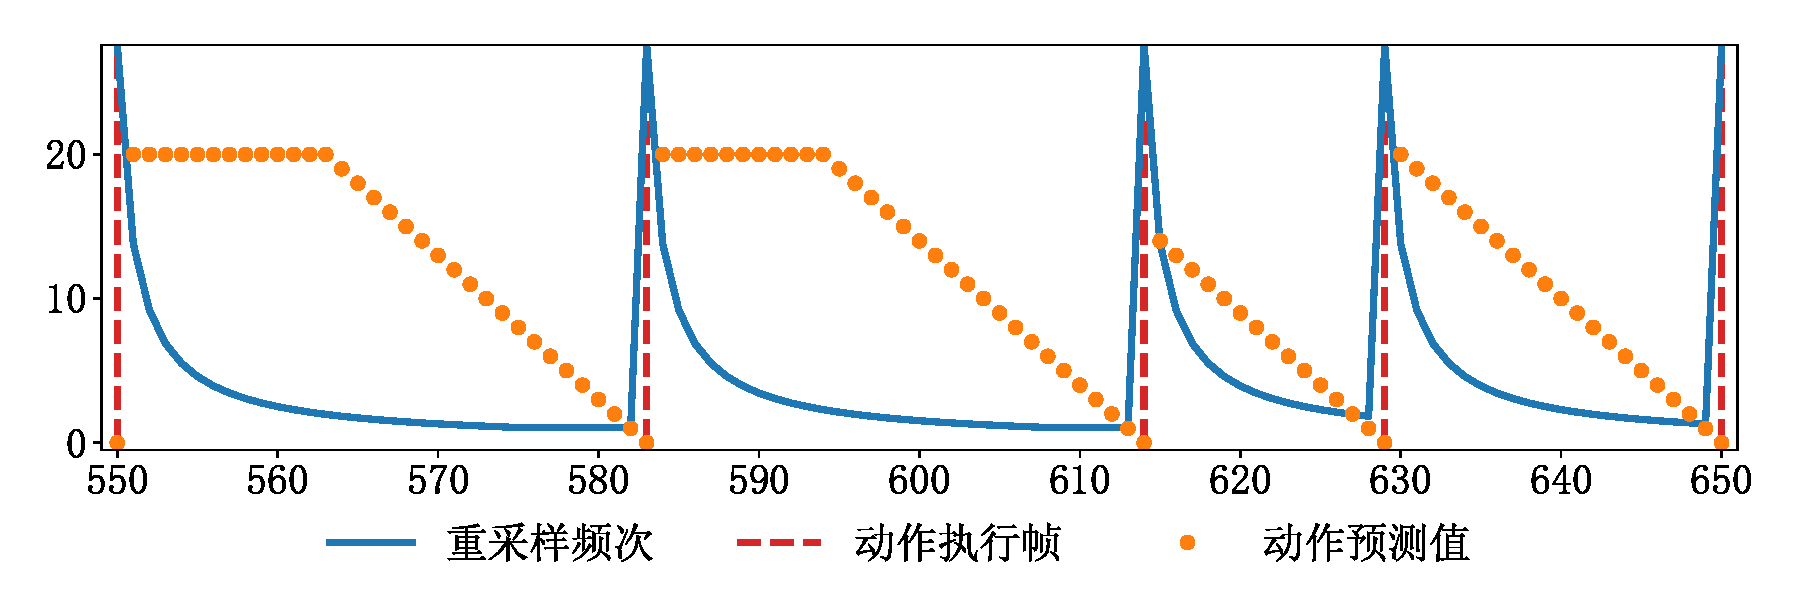
\includegraphics[width=\textwidth]{resample_and_delay.pdf}
  \caption{从离线数据集中截取的一段数据,总共包含5个动作帧,最大间隔帧数阈值$T_{delay} = 20$,}\label{fig-resample-and-delay}
\end{figure}

\BiSubsection{模型架构设计}{}\label{sec-model-struct}
本文设计了3种不同的模型架构,分别基于StARformer和DT模型,
假设输入的轨迹长度为$L$,时序注意力机制中的输入序列长度$T$,使用$N$层Transformer堆叠,
则每种模型架构设计细节如下:

StARformer-3L:基于StARformer架构,
本文设计的StARformer-3L决策模型架构如图~\ref{fig-model}~所示,
其中输入序列长度$T=3L$,第$n$层Transformer输出的时序序列记为
$\{z_t^{img_n},z_t^{card_n},l_{t}^{n-1}\}_{t=1}^{L}$(序列长度$3L$)。
右侧时序注意力机制中的因果Transformer,由于需要使同一时刻下的信息可以相互产生注意力关系,
所以需要引入局部交叉注意力,具体实现方法是将式~\ref{eq-causal-attn}~中的掩码矩阵$M_{3}$,其中$M_{L_0}$定义为
\begin{equation}
  (M_{L_0})_{ij} = \begin{cases}
    1, &\quad i=kL_0-l,j\leqslant kL_0\\
    0, &\quad \text{否则}
  \end{cases},\quad \big(k\in\{1,\cdots,L\}, l\in\{0,\cdots,L_0-1\}\big)
\end{equation}
其本质上是在下三角阵的对角线上顺次放置不交的大小为$L_0\times L_0$的全$1$矩阵。

StARformer-2L:$T=2L$的模型架构与StARformer\upcite{StARformer}论文中架构基本一致,其将图像信息$s_{t}^{img}$与$s_{t}^{card}$编码到同一特征$z_t$中,
得到第$n$层的Transformer输出的时序序列$\{z_t^{n}, l_{t}^{n-1}\}_{t=1}^{L}$(序列长度$2L$),
同理需要使用局部交叉注意力,并将掩码矩阵置为$M_2$,
预测中$a_{t}^{pos}$和$a_{t}^{select}$均使用$z_t$进行解码得到。

DT-4L:基于DT架构,可以看作仅包含图~\ref{fig-model}~中时序注意力部分,
将时序注意力机制中$l_t^{n}$进行替换,得到时序序列为$\{a_{t-1},R_{t-1},s_{t}^{img_n}, s_{t}^{card_n}\}_{t=1}^{L}$(序列长度$4L$),
预测中$a_{t}^{pos}$和$a_{t}^{select}$分别由$s_{t}^{img_n}$和$s_{t}^{card_n}$对应解码得到。

上述各种模型及不同预测目标的验证比对结果请见表~\ref{table-model-eval}~。

\begin{figure}[htbp]
  \centering
  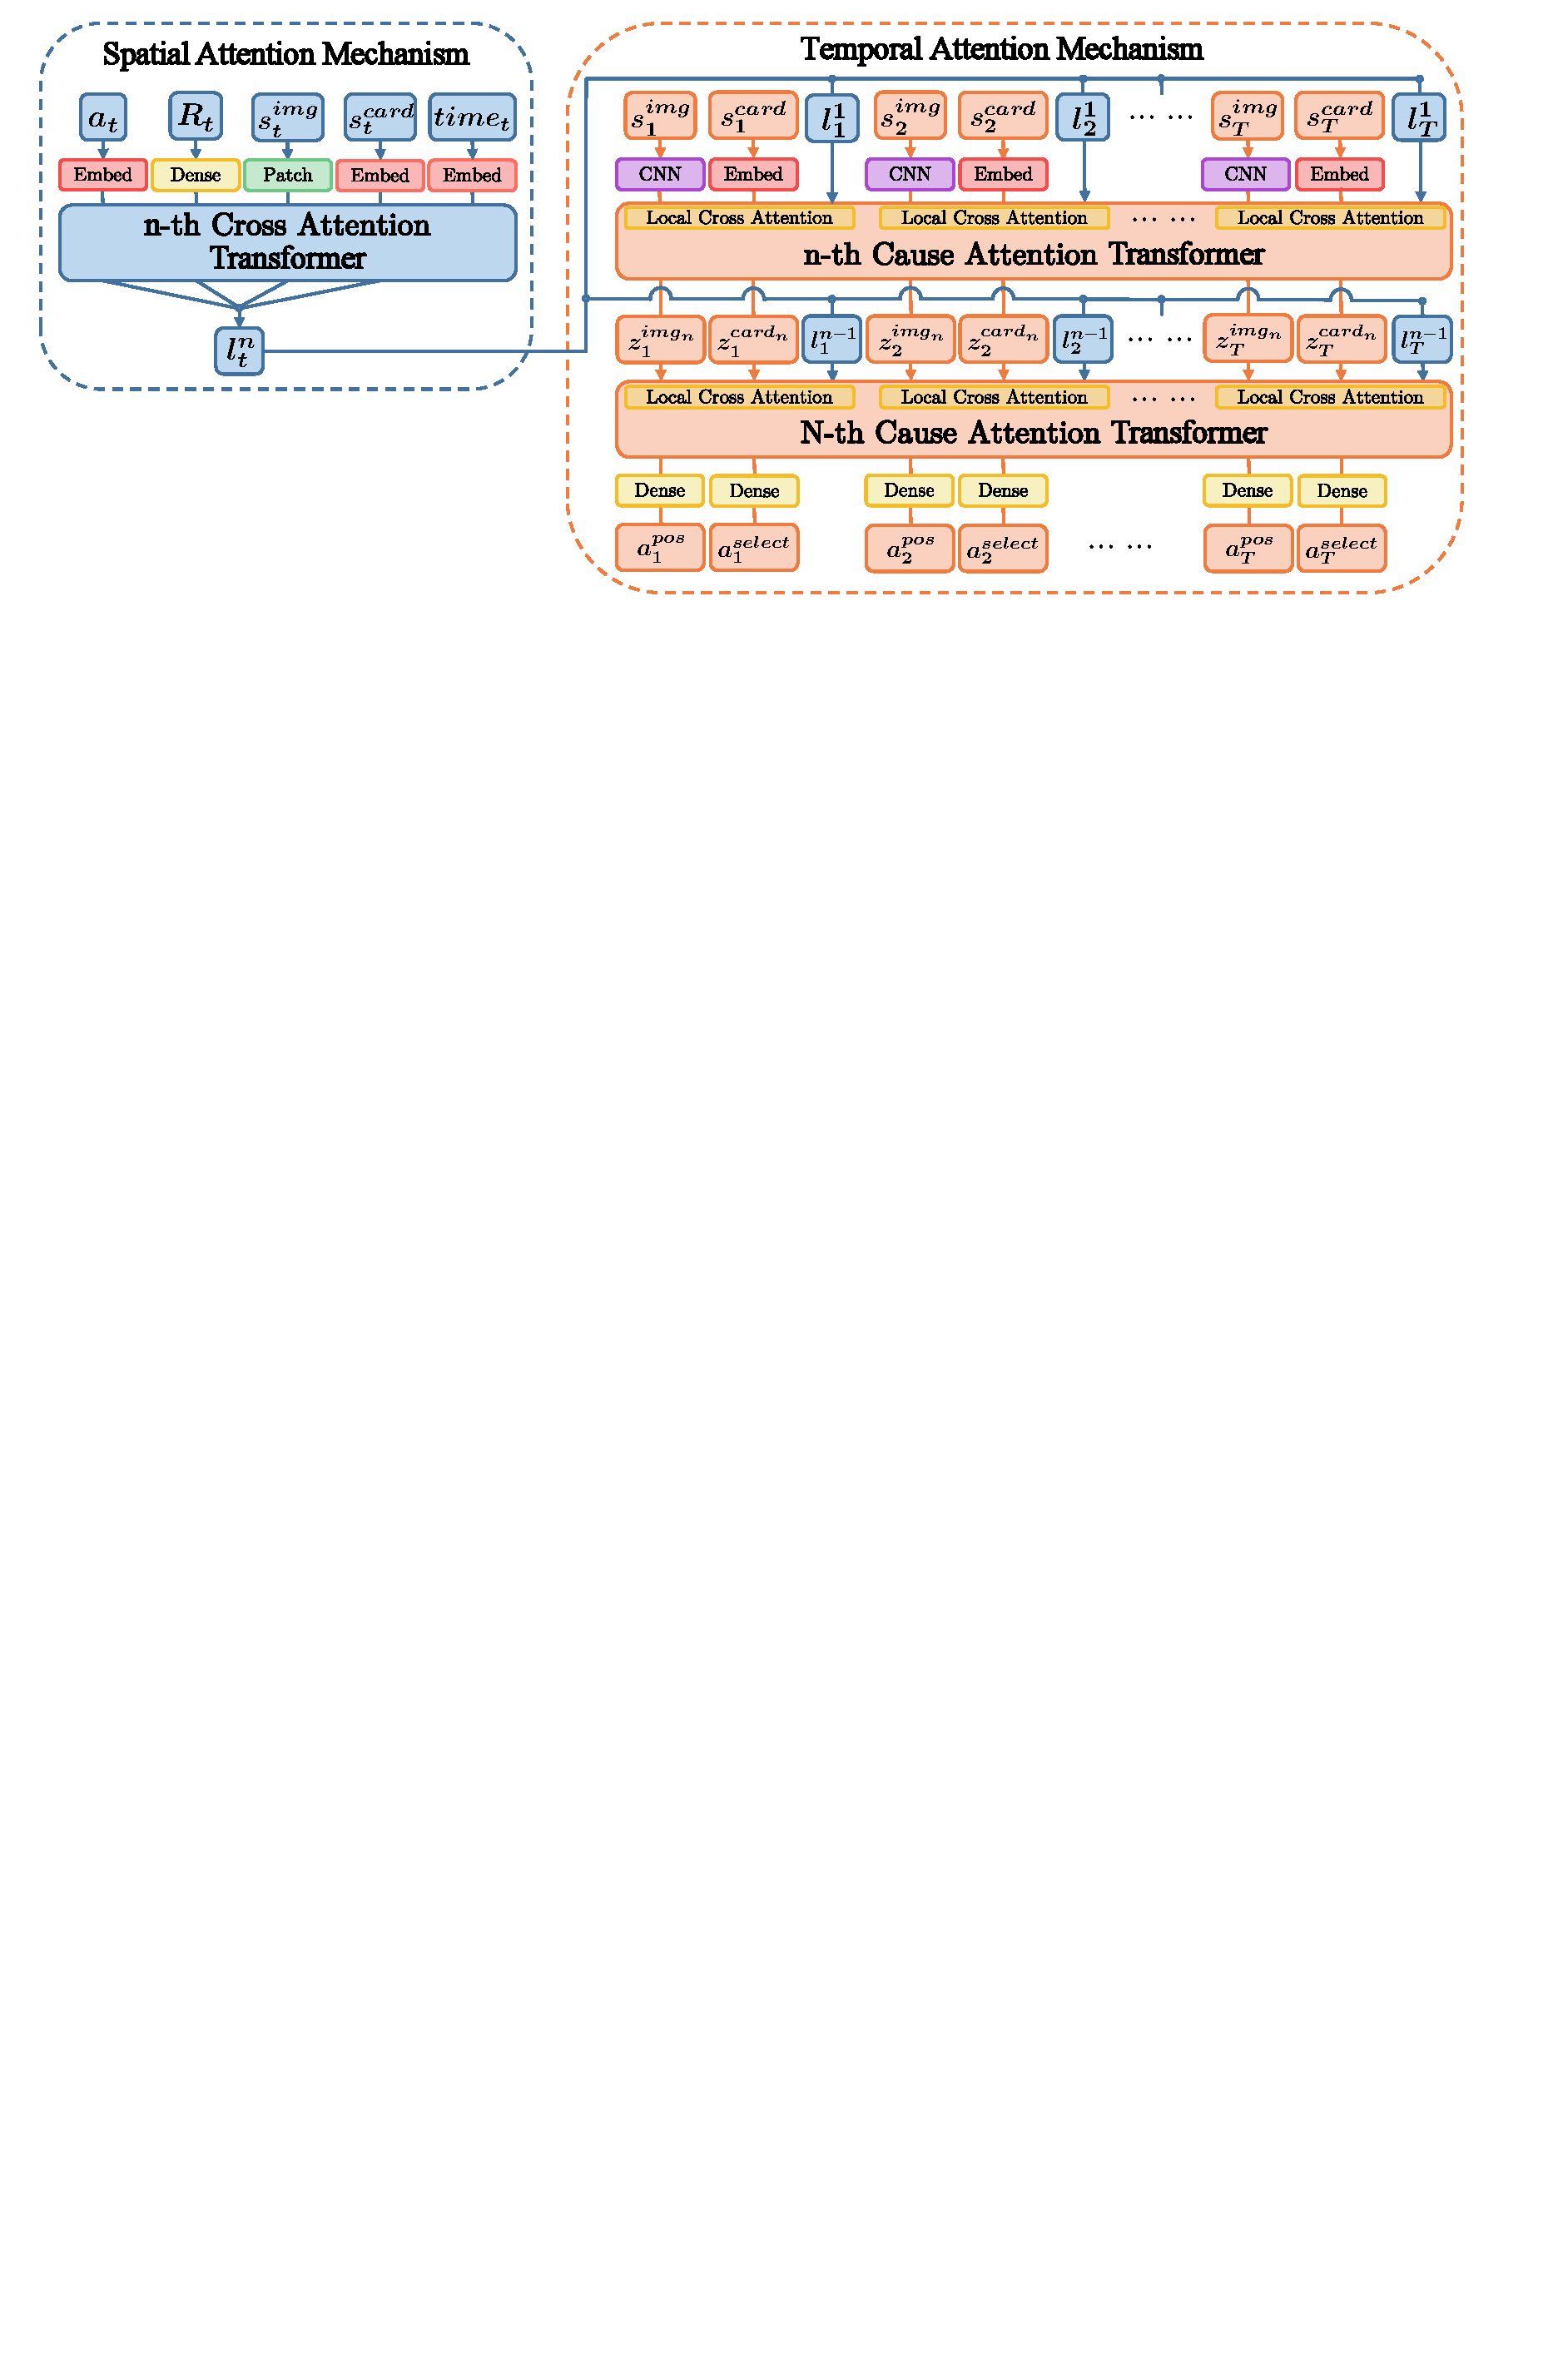
\includegraphics[width=\textwidth]{policy_model.pdf}
  \caption{决策模型:基于StARformer的ViT+DT架构,模型输入为轨迹序列$(a_t, R_t, s_t)_{t=1}^T$,
  输出为动作预测序列$(a_t^{pos},a_t^{select})_{t=1}^T$。左侧交叉注意力机制对
  局部信息$(a_t,R_t,s_t)$按空间维度进行编码,并使用ViT中分块思路将图像$s_t^{img}$转化为序列;
  右侧为因果注意力机制对全局信息$(s^{img}_t,s^{card}_t)$按时序维度进行编码,
  并在每层序列输入中引入对应的局部编码信息$l_t^{n}$。}
  \label{fig-model}
\end{figure}